% =====================================================================
%  Guide utilisateur — Système de Gestion Financière
%  Hôpital de zone de Ménontin
%  Document structuré par profil (chapitres autonomes)
%  Compilation recommandée : tectonic manuel-utilisateur.tex
% =====================================================================
\documentclass[11pt,a4paper]{report}

\usepackage{fontspec}
\usepackage[french]{babel}
\usepackage{graphicx}
\usepackage{float}
\usepackage{xcolor}
\usepackage{tabularx}
\usepackage{booktabs}
\usepackage{array}
\usepackage{longtable}
\usepackage{enumitem}
\usepackage{titlesec}
\usepackage{fancyhdr}
\usepackage{geometry}
\usepackage{titling}
\usepackage[hidelinks]{hyperref}

\geometry{margin=2.4cm}

% ----- Palette (alignée sur l'identité visuelle de l'application) -----
\definecolor{primary}{HTML}{1C6FB8}
\definecolor{accent}{HTML}{409EFF}
\definecolor{darknavy}{HTML}{001529}
\definecolor{success}{HTML}{2E9E5B}
\definecolor{warn}{HTML}{C9821B}
\definecolor{danger}{HTML}{C0392B}
\definecolor{lightbg}{HTML}{EEF2F7}
\definecolor{greytext}{HTML}{5A6675}

% ----- Mise en forme des titres -----
\titleformat{\chapter}[display]
  {\normalfont\huge\bfseries\color{primary}}
  {\flushright\normalsize\color{greytext}\MakeUppercase{\chaptertitlename}\ \thechapter}
  {6pt}{\Huge}
\titlespacing*{\chapter}{0pt}{10pt}{26pt}

\titleformat{\section}
  {\normalfont\Large\bfseries\color{darknavy}}{\thesection}{0.6em}{}
\titleformat{\subsection}
  {\normalfont\large\bfseries\color{primary}}{\thesubsection}{0.6em}{}
\titleformat{\subsubsection}
  {\normalfont\normalsize\bfseries\color{darknavy}}{}{0em}{}

% ----- En-têtes / pieds de page -----
\pagestyle{fancy}
\fancyhf{}
\renewcommand{\headrulewidth}{0.4pt}
\fancyhead[L]{\small\color{greytext}Guide utilisateur}
\fancyhead[R]{\small\color{greytext}\leftmark}
\fancyfoot[C]{\small\color{greytext}\thepage}

% ----- Listes plus aérées -----
\setlist[itemize]{leftmargin=1.4em,itemsep=2pt,topsep=3pt}
\setlist[enumerate]{leftmargin=1.6em,itemsep=2pt,topsep=3pt}

% ----- Emplacement réservé pour une capture d'écran -----
% L'image est volontairement générique : la LÉGENDE décrit
% précisément la capture à insérer pour le processus concerné.
\newcommand{\capture}[1]{%
  \begin{figure}[H]
    \centering
    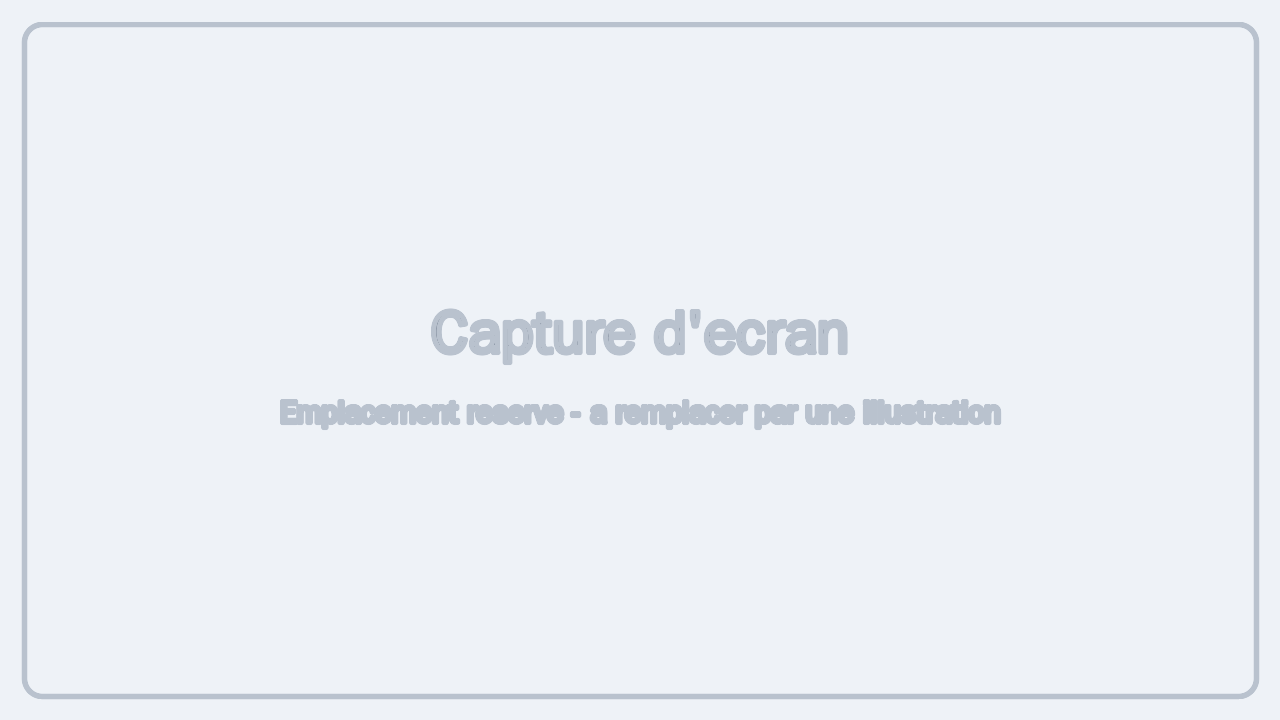
\includegraphics[width=0.82\textwidth]{images/placeholder.png}
    \caption{#1}
  \end{figure}%
}

% ----- Encarts (rendus simples, compatibles export Word) -----
\newcommand{\note}[1]{\par\smallskip\noindent\textbf{\textcolor{primary}{Bon à savoir —}} #1\par\smallskip}
\newcommand{\astuce}[1]{\par\smallskip\noindent\textbf{\textcolor{success}{Astuce —}} #1\par\smallskip}
\newcommand{\attention}[1]{\par\smallskip\noindent\textbf{\textcolor{danger}{Attention —}} #1\par\smallskip}

% ----- Raccourcis -----
\newcommand{\menu}[1]{\textsf{\textbf{#1}}}      % chemin de menu / libellé d'écran
\newcommand{\bouton}[1]{\textsf{[\,#1\,]}}        % bouton cliquable
\newcommand{\champ}[1]{\textit{#1}}                % nom de champ

\setlength{\parskip}{0.5em}
\setlength{\parindent}{0pt}

\hypersetup{
  pdftitle={Guide utilisateur — Hôpital de zone de Ménontin},
  pdfauthor={Hôpital de zone de Ménontin},
}

% =====================================================================
\begin{document}

% ---------------------------- PAGE DE TITRE ----------------------------
\begin{titlepage}
\centering
\vspace*{2.2cm}
{\color{primary}\rule{\textwidth}{2pt}}\\[1.2cm]
{\Huge\bfseries\color{darknavy} Guide de l'utilisateur\par}
\vspace{0.6cm}
{\LARGE Système de Gestion Financière\par}
\vspace{1.4cm}
{\Large\bfseries Hôpital de zone de Ménontin\par}
\vspace{0.4cm}
{\large\color{greytext} République du Bénin\par}
\vspace{2.2cm}
{\large Manuel d'utilisation organisé par profil\par}
\vspace{0.3cm}
{\color{greytext} Administrateur \textbullet{} Comptable \textbullet{} Gestionnaire \textbullet{} Utilisateur\par}
\vfill
{\color{primary}\rule{\textwidth}{2pt}}\\[0.5cm]
{\color{greytext} Document de référence — à compléter avec les captures d'écran de l'application\par}
\end{titlepage}

% ---------------------------- TABLE DES MATIÈRES ----------------------
\tableofcontents
\thispagestyle{empty}
\clearpage

% =====================================================================
\chapter{Prise en main}
% =====================================================================

Ce chapitre s'adresse à \emph{tous} les utilisateurs, quel que soit leur profil. Il décrit comment accéder à l'application, s'y connecter, se repérer dans l'interface, gérer son compte personnel et se déconnecter. Les chapitres suivants détaillent ensuite, profil par profil, l'ensemble des actions disponibles.

\section{À propos de ce guide}

L'application de gestion financière de l'Hôpital de zone de Ménontin permet de suivre l'ensemble des opérations comptables et financières de l'établissement~: fournisseurs et factures d'achat, clients et factures de prestations, règlements, avances, trésorerie (banques et caisses), plan comptable et états de synthèse (rapports).

Chaque personne se connecte avec un \textbf{profil} qui détermine précisément ce qu'elle a le droit de voir et de faire. Ce guide consacre un chapitre complet et autonome à chacun des quatre profils~:

\begin{itemize}
  \item \textbf{Administrateur} — accès total, y compris l'administration (utilisateurs, rôles, paramètres, journal).
  \item \textbf{Comptable} — saisie et suivi complets des opérations (création et modification), validation des factures, consultation des rapports.
  \item \textbf{Gestionnaire} — consultation des données et des rapports, sans saisie.
  \item \textbf{Utilisateur} — consultation des données opérationnelles, sans rapports ni administration.
\end{itemize}

\note{Vous pouvez lire directement le chapitre correspondant à votre profil~: il est complet et se suffit à lui-même. Reportez-vous au présent chapitre pour tout ce qui concerne la connexion, la navigation générale et la gestion de votre compte.}

\subsection*{Conventions de lecture}

\begin{itemize}
  \item \bouton{Libellé} désigne un bouton sur lequel cliquer.
  \item \menu{Libellé} désigne un élément de menu ou un titre d'écran.
  \item \champ{Libellé} désigne un champ de formulaire à renseigner.
  \item Les montants sont exprimés en francs CFA (XOF), sans décimale, avec séparateur de milliers (par exemple \og 1\,250\,000 F\fg{}).
  \item Les dates sont affichées et saisies au format jour/mois/année (JJ/MM/AAAA).
  \item Chaque processus important est accompagné d'un \emph{emplacement réservé à une capture d'écran}~: la légende indique l'illustration à insérer.
\end{itemize}

\section{Accès et connexion}

L'application s'utilise depuis un navigateur web (Google Chrome, Mozilla Firefox, Microsoft Edge\ldots), à l'adresse fournie par l'administrateur de l'établissement. À l'ouverture, vous êtes automatiquement dirigé vers l'écran de connexion tant que vous n'êtes pas authentifié.

\subsection{Se connecter}

L'écran de connexion présente, à gauche, le formulaire de connexion et, à droite, une présentation de l'application.

Pour vous connecter~:

\begin{enumerate}
  \item Saisissez votre \champ{Adresse e-mail} dans le premier champ.
  \item Saisissez votre \champ{Mot de passe}. Le bouton en forme d'œil situé dans le champ permet d'\emph{afficher} ou de \emph{masquer} les caractères saisis, afin de vérifier votre saisie.
  \item Cochez éventuellement \champ{Se souvenir de moi} pour rester connecté plus longtemps sur cet ordinateur.
  \item Cliquez sur \bouton{Se connecter}. Pendant la vérification, le bouton affiche un indicateur de chargement.
\end{enumerate}

Si l'adresse e-mail ou le mot de passe est incorrect, un message d'erreur s'affiche et vous pouvez corriger votre saisie. Le mot de passe doit comporter au moins six caractères. Une fois connecté, vous arrivez sur le \menu{Tableau de bord}.

\attention{Si votre compte a été désactivé par un administrateur, la connexion est refusée même avec le bon mot de passe. Rapprochez-vous de l'administrateur de l'établissement.}

\capture{Écran de connexion~: champs Adresse e-mail et Mot de passe, case \og Se souvenir de moi \fg{} et bouton \og Se connecter \fg{}.}

\section{Découvrir l'interface}

Une fois connecté, l'écran se compose de trois zones permanentes~: le \textbf{menu latéral} (à gauche), la \textbf{barre supérieure} (en haut) et la \textbf{zone de travail} (au centre).

\subsection{Le menu latéral}

Le menu latéral, sur fond bleu nuit, donne accès aux différents modules. Son contenu s'adapte automatiquement à votre profil~: vous ne voyez que les rubriques auxquelles vous avez droit. Les rubriques sont regroupées par thème~:

\begin{itemize}
  \item \menu{Tableau de bord} — la page d'accueil avec les indicateurs clés.
  \item \menu{Factures Fournisseurs} — Fournisseurs, Factures, Règlements.
  \item \menu{Factures Clients} — Clients, Factures, Règlements, Avances.
  \item \menu{Autres} — Plan Comptable, Banques.
  \item \menu{Rapports} — Rapports Fournisseurs, Rapports Clients, Rapports Banques.
  \item \menu{Paramètres} — Utilisateurs, Rôles \& Permissions, Taux Fiscaux, Établissement.
  \item \menu{Journal d'Activité} — l'historique des opérations.
\end{itemize}

Le bouton situé en bas du menu permet de \emph{réduire} ou \emph{déplier} la barre latérale afin d'agrandir la zone de travail.

\capture{Menu latéral déplié montrant les groupes de rubriques (le contenu varie selon le profil connecté).}

\subsection{La barre supérieure}

La barre supérieure affiche, à gauche, un \emph{fil d'Ariane} (breadcrumb) qui rappelle votre position dans l'application. À droite, votre nom et votre avatar ouvrent un menu déroulant proposant~:

\begin{itemize}
  \item \bouton{Mon Profil} — pour consulter et modifier vos informations personnelles~;
  \item \bouton{Déconnexion} — pour quitter l'application en toute sécurité.
\end{itemize}

\subsection{Repères communs à tous les écrans}

La plupart des listes de l'application partagent les mêmes repères, qu'il est utile de connaître une fois pour toutes~:

\begin{itemize}
  \item Des \textbf{cartes de statistiques} en haut de page résument les chiffres importants (totaux, montants payés, restes à payer\ldots).
  \item Un \textbf{champ de recherche} filtre la liste en temps réel à mesure que vous tapez.
  \item Des \textbf{filtres} complémentaires (par exemple par fournisseur, par statut ou par période) affinent l'affichage~; un bouton \bouton{Réinitialiser} efface tous les filtres.
  \item Les tableaux se \textbf{trient} en cliquant sur l'en-tête d'une colonne et se \textbf{paginent} (10, 20, 50 ou 100 lignes par page).
  \item Les actions sur une ligne sont regroupées dans un menu \bouton{\ldots} (\og plus d'actions \fg{}) en bout de ligne.
  \item Toute suppression demande une \textbf{confirmation} avant d'être exécutée.
\end{itemize}

\section{Gérer son compte~: Mon Profil}

L'écran \menu{Mon Profil}, accessible depuis le menu de votre nom en haut à droite, est disponible pour tous les profils. Il se compose d'une carte de présentation à gauche et de deux formulaires à droite.

\subsection{Modifier ses informations personnelles}

Dans le formulaire \menu{Informations personnelles}, vous pouvez mettre à jour votre \champ{Nom complet}, votre \champ{Adresse e-mail}, votre \champ{Téléphone} et votre \champ{Poste}. Cliquez sur \bouton{Enregistrer les modifications} pour valider.

\capture{Écran Mon Profil~: carte de présentation, informations personnelles et changement de mot de passe.}

\subsection{Changer son mot de passe}

Dans le formulaire \menu{Changer le mot de passe}, renseignez votre \champ{Mot de passe actuel}, votre \champ{Nouveau mot de passe} puis sa \champ{Confirmation}, et cliquez sur \bouton{Changer le mot de passe}. Pour des raisons de sécurité, le nouveau mot de passe doit contenir au moins huit caractères mêlant minuscules, majuscules, chiffres et caractère spécial. Un message vous prévient si le mot de passe actuel est incorrect ou si la confirmation ne correspond pas.

\subsection{Gérer sa signature}

La carte \menu{Ma signature} permet de téléverser une image de votre signature manuscrite (au format PNG ou JPG, jusqu'à 2~Mo). Cette signature pourra être reprise sur certains documents officiels. Utilisez \bouton{Ajouter une signature} (ou \bouton{Changer la signature} si une signature existe déjà), et \bouton{Supprimer} pour la retirer.

\capture{Carte Ma signature~: aperçu de la signature téléversée et boutons d'ajout / suppression.}

\section{Se déconnecter}

\subsection{Déconnexion manuelle}

Pour quitter l'application, ouvrez le menu de votre nom en haut à droite et cliquez sur \bouton{Déconnexion}. Vous êtes alors ramené à l'écran de connexion.

\subsection{Déconnexion automatique en cas d'inactivité}

Par sécurité, l'application vous déconnecte automatiquement après une période d'inactivité. Au bout d'environ quatorze minutes sans action (ni clic, ni frappe au clavier, ni déplacement de la souris), une fenêtre \menu{Session bientôt expirée} vous prévient que la déconnexion interviendra dans une minute. Vous pouvez alors cliquer sur \bouton{Rester connecté} pour prolonger votre session, ou sur \bouton{Se déconnecter} pour quitter immédiatement. Sans réponse de votre part, la déconnexion est automatique.

\attention{Pensez à enregistrer régulièrement votre travail (validation des formulaires) pour ne rien perdre en cas de déconnexion automatique.}

% =====================================================================
\chapter{Profil Administrateur}
% =====================================================================

L'\textbf{Administrateur} dispose de l'accès le plus complet à l'application. Il peut réaliser toutes les opérations métier (fournisseurs, clients, factures, règlements, avances, trésorerie, comptabilité), consulter et exporter tous les rapports, et il est le seul à accéder à l'\emph{administration}~: gestion des utilisateurs, des rôles et permissions, des paramètres fiscaux, des informations de l'établissement et du journal d'activité.

\section{Périmètre du profil}

Le tableau ci-dessous récapitule ce que l'Administrateur peut faire dans chaque module.

\renewcommand{\arraystretch}{1.3}
\begin{longtable}{>{\raggedright\arraybackslash}p{5.4cm} >{\raggedright\arraybackslash}p{9.2cm}}
\toprule
\textbf{Module} & \textbf{Droits de l'Administrateur} \\
\midrule
\endhead
Fournisseurs & Consulter, créer, modifier, supprimer \\
Factures fournisseurs & Consulter, créer, modifier, valider, solder, supprimer \\
Règlements fournisseurs & Consulter, créer, modifier, supprimer \\
Clients & Consulter, créer, modifier, supprimer \\
Factures clients & Consulter, créer, modifier, solder, supprimer \\
Règlements clients & Consulter, créer, modifier, supprimer \\
Avances clients & Consulter, créer, modifier, supprimer \\
Plan comptable & Consulter, créer, modifier, supprimer \\
Banques \& trésorerie & Consulter, créer, approvisionner, modifier, supprimer \\
Rapports & Consulter et exporter (PDF / Excel) \\
Paramètres (taux fiscaux, établissement) & Consulter et modifier \\
Utilisateurs & Consulter, créer, modifier, activer/désactiver, supprimer \\
Rôles \& permissions & Consulter, créer, modifier, supprimer \\
Journal d'activité & Consulter \\
\bottomrule
\end{longtable}
\renewcommand{\arraystretch}{1}

\section{Le tableau de bord}

À la connexion, l'Administrateur arrive sur le \menu{Tableau de bord}, qui offre une vue d'ensemble de la santé financière de l'établissement.

En haut, quatre indicateurs clés sont présentés sous forme de cartes~:

\begin{itemize}
  \item \menu{Chiffre d'affaires} — le montant facturé aux clients sur le mois en cours, avec l'évolution en pourcentage par rapport au mois précédent.
  \item \menu{Factures en attente} — le nombre de factures non soldées, réparties entre clients et fournisseurs.
  \item \menu{Dettes fournisseurs} — le total restant à payer aux fournisseurs.
  \item \menu{Créances clients} — le total restant à encaisser auprès des clients.
\end{itemize}

En dessous, l'écran présente le tableau des \menu{Dernières factures fournisseurs} (numéro, fournisseur, montant, date, statut) avec un bouton \bouton{Voir tout} renvoyant vers la liste complète, ainsi qu'une carte \menu{Situation des banques} listant chaque compte avec son solde et le solde total. Deux graphiques complètent la page~: l'\menu{Évolution mensuelle} des recettes et dépenses sur douze mois, et la \menu{Répartition des charges} par fournisseur sur l'année.

\capture{Tableau de bord~: les quatre cartes d'indicateurs, le tableau des dernières factures, la situation des banques et les deux graphiques.}

\section{Gérer les fournisseurs}

Le module \menu{Fournisseurs} centralise les tiers auprès desquels l'hôpital effectue ses achats. On y accède par \menu{Factures Fournisseurs > Fournisseurs}.

\subsection{Consulter et rechercher}

La liste affiche, pour chaque fournisseur, sa raison sociale, son type (Médicaments, Équipements, Consommables, Services, Maintenance, Autres), son compte comptable, son contact, son téléphone et son e-mail. Une carte indique le nombre total de fournisseurs. Vous pouvez rechercher un fournisseur par code, nom, compte, e-mail ou téléphone, ou filtrer par compte comptable.

\capture{Liste des fournisseurs avec la carte de total, le champ de recherche et le filtre par compte comptable.}

\subsection{Créer un fournisseur}

Cliquez sur \bouton{Nouveau Fournisseur} pour ouvrir le formulaire, organisé en onglets~:

\begin{enumerate}
  \item \menu{Informations générales} — saisissez la \champ{Raison sociale} (obligatoire) et choisissez le \champ{Type de fournisseur}.
  \item \menu{Coordonnées} — renseignez le contact, sa fonction, les téléphones, l'e-mail, le site web, l'adresse, la ville et le pays.
  \item \menu{Compte comptable} — chaque fournisseur possède son propre compte auxiliaire. Vous pouvez \emph{sélectionner un compte existant} (classe 401 ou 4812) ou \emph{créer un nouveau compte}~: choisissez le compte parent, saisissez (ou générez automatiquement via le bouton \bouton{Auto}) le numéro de compte, et indiquez son libellé (par défaut, le nom du fournisseur).
  \item \menu{Informations fiscales} — saisissez l'\champ{IFU} (treize chiffres, obligatoire) et le \champ{RCCM}.
  \item \menu{Complémentaires} — ajoutez d'éventuelles observations.
\end{enumerate}

Naviguez avec \bouton{Précédent} et \bouton{Suivant}, puis cliquez sur \bouton{Enregistrer}. Un message confirme la création.

\capture{Formulaire de création d'un fournisseur~: onglet Informations générales et onglet Compte comptable.}

\subsection{Consulter la fiche d'un fournisseur}

Depuis la liste, l'action \bouton{Voir} ouvre la fiche détaillée, organisée en trois onglets~: \menu{Informations} (coordonnées, informations fiscales, observations, historique de création), \menu{Factures} (toutes les factures du fournisseur, avec montant, payé, reste et statut) et \menu{Règlements} (l'historique des paiements, avec accès aux bordereaux et fiches d'imputation). Des cartes statistiques affichent le nombre de factures, le total facturé, le montant payé et le reste à payer.

\capture{Fiche fournisseur~: cartes statistiques et onglets Informations / Factures / Règlements.}

\subsection{Modifier et supprimer}

L'action \bouton{Modifier} (depuis la liste ou la fiche) rouvre le formulaire pré-rempli. L'action \bouton{Supprimer} retire le fournisseur après confirmation.

\section{Gérer les factures fournisseurs}

Le module \menu{Factures Fournisseurs > Factures} permet d'enregistrer et de suivre les factures d'achat.

\subsection{Consulter et filtrer}

La liste présente le numéro de pièce, la date, le fournisseur, la référence, le libellé, le montant TTC, le net à payer, le montant déjà payé et le statut. Quatre cartes résument le total des factures et les montants impayés, partiellement payés et payés. Vous pouvez rechercher par numéro ou référence, et filtrer par fournisseur, par statut de paiement (Impayée, Partielle, Payée) ou par période.

\capture{Liste des factures fournisseurs~: cartes de synthèse, filtres et tableau des factures.}

\subsection{Créer une facture}

Cliquez sur \bouton{Nouvelle Facture}. Le formulaire se présente en quatre onglets~:

\begin{enumerate}
  \item \menu{Informations} — saisissez le \champ{N° de pièce} (le bouton \bouton{Auto} le génère et vérifie qu'il n'existe pas déjà), la \champ{Date d'enregistrement}, la \champ{Référence / N° de bon de commande}, sa date, le \champ{Fournisseur} et le \champ{Libellé}.
  \item \menu{Montants} — précisez si la facture est \champ{assujettie à la TVA} et son taux, le \champ{Montant HT}, un éventuel \champ{Avoir}, le \champ{Montant main-d'œuvre} (base de l'AIB), le compte et le \champ{taux d'AIB}. Un récapitulatif calcule en temps réel le HT, la TVA, l'AIB, le TTC et le net à payer.
  \item \menu{Imputations comptables} — répartissez les \emph{débits} (charges, immobilisations, personnel) qui doivent totaliser le HT, et les \emph{crédits} (comptes fournisseurs) qui doivent totaliser le TTC. Chaque ligne précise l'imputation, le compte, le libellé et le montant~; un repère de couleur indique si le total saisi correspond à la cible.
  \item \menu{Observations} — ajoutez vos notes.
\end{enumerate}

Cliquez sur \bouton{Enregistrer}.

\note{La cohérence comptable est contrôlée~: la somme des débits doit égaler le montant HT et la somme des crédits le montant TTC.}

\capture{Formulaire de facture fournisseur~: onglet Montants (calcul automatique TVA/AIB/TTC) et onglet Imputations comptables.}

\subsection{Consulter le détail d'une facture}

L'action \bouton{Voir} ouvre la fiche de la facture~: informations générales, imputations (débits et crédits), montants détaillés, récapitulatif financier avec barre de progression du paiement, et historique des règlements. Des badges indiquent le statut de paiement et l'état de l'imputation comptable.

\capture{Détail d'une facture fournisseur~: récapitulatif financier, barre de progression et historique des règlements.}

\subsection{Valider l'imputation, solder, modifier, supprimer}

Depuis la fiche ou le menu d'actions de la liste, l'Administrateur peut~:

\begin{itemize}
  \item \bouton{Marquer comme soldée} — clôturer manuellement une facture (après confirmation), même sans règlement intégral.
  \item Générer les écritures d'\bouton{Imputation comptable} et les consulter dans un panneau latéral, avec téléchargement en PDF.
  \item Ouvrir l'\bouton{État de règlement} de la facture (panneau latéral + PDF).
  \item \bouton{Modifier} la facture ou la \bouton{Supprimer} (après confirmation).
\end{itemize}

\capture{Panneau d'imputation comptable d'une facture, avec le bouton de téléchargement PDF.}

\subsection{Régler une facture fournisseur}

L'action \bouton{Régler} ouvre la page de règlement. Le côté gauche rappelle les informations et les montants de la facture ainsi que l'historique des paiements~; le côté droit contient le formulaire~:

\begin{enumerate}
  \item Choisissez l'\champ{Année d'exercice} et la \champ{Date de règlement}.
  \item Si la facture comporte une imputation détaillée, répartissez le montant à solder par compte fournisseur dans le tableau (bouton \bouton{Ajouter un compte}), sinon saisissez directement le \champ{Montant payé}.
  \item Sélectionnez le \champ{Mode de paiement}~: \emph{Espèces}, \emph{Chèque} ou \emph{Virement}. Pour un chèque ou un virement, indiquez la \champ{Banque}, le \champ{Compte bancaire}, la \champ{Référence} et sa date~; le solde du compte s'affiche pour information.
  \item Indiquez le \champ{Bénéficiaire} (avec suggestions), cochez le cas échéant \champ{Déclarer l'AIB}, et ajoutez vos \champ{Notes}.
  \item Un récapitulatif détaille le total à solder, la retenue AIB éventuelle et le décaissement réel. Cliquez sur \bouton{Enregistrer le règlement}.
\end{enumerate}

\attention{Si le solde du compte bancaire est insuffisant, une fenêtre demande explicitement votre autorisation avant d'enregistrer le règlement.}

\capture{Page de règlement d'une facture fournisseur~: répartition par compte, mode de paiement et récapitulatif du décaissement.}

\section{Suivre les règlements fournisseurs}

Le module \menu{Factures Fournisseurs > Règlements} présente tous les règlements, regroupés par facture. Quatre cartes affichent le total des règlements, le montant du mois, le nombre de règlements et le montant moyen. Vous pouvez filtrer par fournisseur, mode de paiement et période.

Chaque ligne de facture se déplie pour révéler le détail des règlements (date, mode, référence, bénéficiaire, compte bancaire, auteur de la saisie, montant). Pour chaque règlement, le menu d'actions permet de générer le \bouton{Bordereau} (PDF), la fiche d'\bouton{Imputation} (PDF, sauf espèces), de \bouton{Modifier} ou de \bouton{Supprimer} le règlement. Le bouton \bouton{Nouveau Règlement} ouvre une fenêtre de sélection d'une facture impayée pour démarrer un règlement.

\capture{Liste des règlements fournisseurs regroupés par facture, avec le détail déplié et les actions PDF.}

\section{Gérer les clients}

Le module \menu{Factures Clients > Clients} recense les tiers facturés par l'hôpital. La liste affiche le numéro de compte, la raison sociale, le téléphone et l'adresse, avec une carte indiquant le nombre total de clients et un champ de recherche.

\subsection{Créer ou modifier un client}

Le bouton \bouton{Nouveau Client} ouvre une fenêtre à deux onglets~:

\begin{enumerate}
  \item \menu{Informations} — \champ{Raison sociale} (obligatoire), \champ{Téléphone}, \champ{IFU} (treize chiffres), \champ{Type de client} (Société, Divers, Personnel, Autre), \champ{Adresse} et \champ{Observation}.
  \item \menu{Compte comptable} — sélectionnez un compte client existant (classe 41) ou créez-en un nouveau (compte parent, numéro avec génération \bouton{Auto}, libellé).
\end{enumerate}

Cliquez sur \bouton{Enregistrer}. L'action \bouton{Modifier} rouvre ce formulaire, \bouton{Voir les factures} renvoie vers les factures du client et \bouton{Supprimer} retire le client après confirmation.

\capture{Fenêtre de création d'un client~: onglet Informations et onglet Compte comptable.}

\section{Gérer les factures clients}

Le module \menu{Factures Clients > Factures} permet d'émettre et de suivre les factures de prestations. La liste affiche la référence, la date, le client, le montant, le payé, le reste et le statut~; quatre cartes synthétisent le total facturé, payé et les créances. Vous pouvez filtrer par client, statut et période.

\subsection{Créer une facture client}

Le bouton \bouton{Nouvelle Facture} ouvre une fenêtre où vous saisissez la \champ{Référence} (bouton \bouton{Auto} disponible), la \champ{Date}, le \champ{Client}, le \champ{Montant} et une éventuelle \champ{Ristourne}~; le \emph{net à payer} est calculé automatiquement. Cliquez sur \bouton{Enregistrer}.

\capture{Fenêtre de création d'une facture client avec calcul automatique du net à payer.}

\subsection{Consulter, solder, modifier, supprimer}

L'action \bouton{Voir} ouvre la fiche de la facture (informations, récapitulatif, barre de progression du paiement). Tant que la facture n'est pas payée, vous pouvez \bouton{Enregistrer un règlement} ou la \bouton{Marquer comme soldée}. Les actions \bouton{Modifier} et \bouton{Supprimer} sont également disponibles.

\capture{Détail d'une facture client~: récapitulatif et barre de progression du paiement.}

\subsection{Régler une facture client}

L'action \bouton{Régler} ouvre la page de règlement. Le côté gauche rappelle les informations de la facture et l'historique des règlements~; le côté droit contient le formulaire~:

\begin{enumerate}
  \item Le \champ{N° de ligne} est attribué automatiquement. Choisissez le \champ{Type}~: \emph{Règlement} ou \emph{Perte}.
  \item Pour un règlement, saisissez le \champ{Montant} et, le cas échéant, un \champ{Montant rejeté} (chèque rejeté).
  \item Choisissez la \emph{source du paiement}~: un \textbf{paiement direct} (institution, référence de chèque, banque de dépôt, référence de bordereau, et téléversement du bordereau de dépôt) ou l'\textbf{imputation sur une avance} disponible du client.
  \item Ajoutez vos \champ{Notes}. Un récapitulatif affiche le montant et le nouveau reste à payer, puis cliquez sur \bouton{Enregistrer le règlement}.
\end{enumerate}

\capture{Page de règlement d'une facture client~: type de règlement, source du paiement et dépôt bancaire.}

\section{Suivre les règlements clients}

Le module \menu{Factures Clients > Règlements} présente tous les règlements clients, regroupés par facture (avec détail dépliable). Quatre cartes affichent le total, le montant du mois, le nombre et le montant moyen. Vous pouvez filtrer par client, type et période, consulter le détail d'un règlement, le modifier ou le supprimer, et démarrer un \bouton{Nouveau Règlement} en sélectionnant une facture.

\capture{Liste des règlements clients regroupés par facture.}

\section{Gérer les avances clients}

Le module \menu{Factures Clients > Avances} gère les chèques d'avance reçus de tiers (par exemple des assurances) et leur consommation. Quatre cartes affichent le total des avances reçues, le total consommé, le solde disponible et le nombre d'avances. La liste précise pour chaque avance la société émettrice, le numéro de chèque, le montant, la part utilisée, le solde et le statut (Disponible, Partiellement utilisée, Épuisée).

Le bouton \bouton{Nouvelle avance} ouvre un formulaire~: \champ{Client bénéficiaire}, \champ{Société émettrice}, \champ{N° de chèque}, \champ{Date du chèque}, \champ{Montant}, éventuellement \champ{N° de proforma}, \champ{Institution}, \champ{Banque de dépôt}, \champ{Référence de bordereau} et téléversement du \champ{Bordereau de dépôt}. Une avance se consomme ensuite lors du règlement d'une facture client (option \emph{imputation sur une avance}). Les actions \bouton{Détails}, \bouton{Modifier} et \bouton{Supprimer} (uniquement si l'avance n'a pas encore été utilisée) sont disponibles.

\capture{Liste des avances clients et fenêtre de création d'une avance.}

\section{Tenir le plan comptable}

Le module \menu{Autres > Plan Comptable} gère la nomenclature comptable OHADA (classes 1 à 8). Huit cartes répartissent les comptes par classe (Capitaux, Immobilisations, Stocks, Tiers, Trésorerie, Charges, Produits\ldots) et la liste affiche le numéro, le libellé, la classe et une marque \og Personnalisé \fg{} pour les comptes ajoutés manuellement. Vous pouvez rechercher par numéro ou libellé et filtrer par classe ou par source (OHADA standard / personnalisé).

Le bouton \bouton{Nouveau Compte} ouvre un formulaire~: \champ{Compte parent} (facultatif), \champ{Numéro de compte} et \champ{Libellé}. Les comptes personnalisés peuvent être \bouton{Modifiés} et \bouton{Supprimés} (après confirmation)~; les comptes standard OHADA ne sont pas supprimables.

\capture{Plan comptable OHADA~: cartes par classe, liste des comptes et fenêtre d'ajout de compte.}

\section{Gérer les banques et la trésorerie}

Le module \menu{Autres > Banques} suit les comptes bancaires et les caisses de l'établissement. La page affiche le solde global, les entrées et sorties du mois, la liste des banques (en colonne de gauche) et les comptes de la banque sélectionnée (sous forme de cartes avec leur solde).

\subsection{Créer une banque et un compte}

Le menu \bouton{Nouveau} propose \bouton{Nouvelle Banque} (il suffit d'indiquer le \champ{Nom}) et \bouton{Nouveau Compte} (\champ{Banque}, \champ{Numéro de compte}, \champ{Compte OHADA} de trésorerie, \champ{Observations}).

\subsection{Approvisionner un compte}

Le bouton \bouton{Approvisionner} enregistre un dépôt~: \champ{Compte à approvisionner}, \champ{Date}, \champ{Montant}, \champ{Origine des fonds} (Recette journalière, Subvention, Donation, Virement interne, Remboursement, Autre), \champ{Référence}, \champ{Description} et \champ{Pièce jointe} facultative. Le nouveau solde est calculé et affiché avant validation.

\subsection{Consulter les mouvements}

Le bouton \bouton{Mouvements} d'un compte ouvre l'historique complet des entrées et sorties (date, type, référence, description, montant, solde après opération, auteur de la saisie), avec filtres par type et période et une fenêtre de \bouton{Détails} pour chaque mouvement.

\capture{Module Banques~: liste des comptes avec soldes, approvisionnement et historique des mouvements.}

\section{Consulter et exporter les rapports}

Le menu \menu{Rapports} donne accès à trois familles d'états, chacun assorti de filtres (période, fournisseur/client, compte, banque, exercice\ldots) et d'options d'export \bouton{PDF}, \bouton{Excel} et \bouton{Imprimer}.

\subsection{Rapports fournisseurs}

\begin{itemize}
  \item \menu{Mouvement des factures} — le détail des factures d'un fournisseur (TTC, avoir, AIB, règlements, solde).
  \item \menu{Situation des fournisseurs} — la synthèse des dettes (tous, par compte ou par fournisseur).
  \item \menu{Factures réglées} — les factures payées sur la période (résumé et détail par fournisseur).
  \item \menu{Factures et soldes} — les factures avec leur solde restant (export Excel).
  \item \menu{Déclaration AIB} — la déclaration des retenues AIB, le bordereau de versement et le point avec la TFU.
  \item \menu{Point périodique des PC} — les pièces comptables enregistrées, regroupées par date.
  \item \menu{Bordereau de transmission} — la sélection de règlements à transmettre (mandats et bordereaux).
  \item \menu{Récapitulatif des charges} et \menu{Récapitulatif des investissements} — les dépenses et immobilisations par compte.
  \item \menu{Déclaration de la TVA} — les factures assujetties et la TVA due.
  \item \menu{Banques par compte} — la synthèse des soldes bancaires (approvisionnements, débits, solde).
\end{itemize}

\subsection{Rapports clients}

\begin{itemize}
  \item \menu{État des règlements} — le suivi des règlements, pertes et rejets.
  \item \menu{État des créances} — les factures non soldées par client.
  \item \menu{Brouillard de chèques} — la conciliation et les imputations comptables côté client.
  \item \menu{Chiffre d'affaires} — le chiffre d'affaires global (théorique / physique) ou par client.
  \item \menu{Pertes \& rejets} — la liste des pertes et des rejets de paiement.
\end{itemize}

\subsection{Rapports banques}

\begin{itemize}
  \item \menu{Situation des banques} — la synthèse des soldes et mouvements (toutes les banques ou une banque, avec solde initial, mouvements et solde final).
\end{itemize}

\capture{Écran de rapports~: choix de l'onglet, filtres de période et boutons d'export PDF / Excel.}

\section{Paramétrer l'application}

\subsection{Taux fiscaux}

Le module \menu{Paramètres > Taux Fiscaux} centralise les taux de TVA et d'AIB. Trois cartes indiquent le nombre de taux de chaque type et le nombre de taux actifs. Pour les AIB, le bouton \bouton{Ajouter AIB} ouvre un formulaire (\champ{Libellé}, \champ{Taux (\%)}, \champ{Actif}, \champ{Par défaut}). Chaque taux peut être modifié, activé/désactivé via un interrupteur, marqué par défaut, et les taux AIB supprimés.

\capture{Paramètres des taux fiscaux~: tableaux TVA et AIB avec interrupteurs d'activation.}

\subsection{Informations de l'établissement}

Le module \menu{Paramètres > Établissement} définit les informations reprises en en-tête des documents et rapports~: \champ{Nom de l'établissement}, \champ{Pays / Entité}, \champ{Adresse}, \champ{Téléphone}, \champ{E-mail} et \champ{Nom du Directeur} (affiché au bas des bordereaux de règlement). Cliquez sur \bouton{Enregistrer les paramètres}.

\capture{Écran des paramètres de l'établissement.}

\section{Administrer les utilisateurs}

Le module \menu{Paramètres > Utilisateurs} permet de gérer les comptes. La liste affiche le nom, l'e-mail, le poste, le téléphone, les rôles, le statut (interrupteur actif/inactif) et les actions.

Le bouton \bouton{Nouvel Utilisateur} ouvre un formulaire~: \champ{Nom complet}, \champ{E-mail}, \champ{Mot de passe} (au moins huit caractères mêlant minuscules, majuscules, chiffres et caractère spécial), \champ{Téléphone}, \champ{Poste}, \champ{Rôles} (un ou plusieurs) et \champ{Statut}. En modification, laissez le mot de passe vide pour le conserver. L'interrupteur de statut active ou désactive instantanément un compte~; la suppression demande confirmation (vous ne pouvez pas supprimer votre propre compte).

\capture{Gestion des utilisateurs~: liste, interrupteur de statut et formulaire de création.}

\section{Gérer les rôles et permissions}

Le module \menu{Paramètres > Rôles \& Permissions} présente une \emph{matrice} croisant les permissions (en lignes, regroupées par module) et les rôles (en colonnes). Cliquer sur une cellule accorde ou retire une permission à un rôle. Des boutons permettent d'appliquer en masse toutes les permissions d'un module à un rôle, ou de tout activer / tout désactiver pour un rôle donné.

Le bouton \bouton{Nouveau Rôle} crée un rôle (il suffit d'indiquer son \champ{Nom}, puis de cocher ses permissions dans la matrice). Chaque rôle peut être \bouton{Modifié} ou \bouton{Supprimé} (impossible s'il est encore attribué à des utilisateurs).

\note{Quatre rôles existent par défaut~: Administrateur, Comptable, Gestionnaire et Utilisateur. Vous pouvez les ajuster ou en créer d'autres selon les besoins de l'établissement.}

\capture{Matrice des rôles et permissions~: lignes par module, colonnes par rôle, cellules à cocher.}

\section{Consulter le journal d'activité}

Le module \menu{Journal d'Activité} trace les opérations sensibles réalisées dans l'application~: créations, modifications et suppressions d'utilisateurs et de rôles, attributions de permissions, mises à jour de profil, connexions et déconnexions, etc. Le tableau affiche la date et l'heure, l'utilisateur, l'action, le module, la description et l'adresse IP. Des filtres permettent de cibler par utilisateur, module, type d'action et plage de dates.

\capture{Journal d'activité~: filtres et tableau des opérations tracées.}

% =====================================================================
\chapter{Profil Comptable}
% =====================================================================

Le \textbf{Comptable} est le profil opérationnel central de l'application. Il assure la saisie et le suivi complets des opérations~: il crée et modifie les fournisseurs, les clients, les factures, les règlements et les avances, valide les factures fournisseurs et consulte l'ensemble des rapports. Il consulte également le plan comptable et la trésorerie. En revanche, il ne supprime aucune donnée et n'accède pas à l'administration (utilisateurs, rôles, paramètres, journal).

\section{Périmètre du profil}

\renewcommand{\arraystretch}{1.3}
\begin{longtable}{>{\raggedright\arraybackslash}p{5.4cm} >{\raggedright\arraybackslash}p{9.2cm}}
\toprule
\textbf{Module} & \textbf{Droits du Comptable} \\
\midrule
\endhead
Fournisseurs & Consulter, créer, modifier \\
Factures fournisseurs & Consulter, créer, modifier, valider, solder \\
Règlements fournisseurs & Consulter, créer, modifier \\
Clients & Consulter, créer, modifier \\
Factures clients & Consulter, créer, modifier, solder \\
Règlements clients & Consulter, créer, modifier \\
Avances clients & Consulter, créer, modifier \\
Plan comptable & Consulter \\
Banques \& trésorerie & Consulter \\
Rapports & Consulter et exporter (PDF / Excel) \\
Paramètres, Utilisateurs, Rôles, Journal & Non accessibles \\
\bottomrule
\end{longtable}
\renewcommand{\arraystretch}{1}

\note{Le Comptable ne dispose pas de l'action \og Supprimer \fg{} sur les fournisseurs, clients, factures, règlements et avances. Pour solder une facture sans paiement intégral, utilisez \bouton{Marquer comme soldée}~; pour annuler un règlement erroné, rapprochez-vous d'un administrateur.}

\section{Le tableau de bord}

À la connexion, le Comptable arrive sur le \menu{Tableau de bord}, qui présente quatre indicateurs clés (chiffre d'affaires du mois, factures en attente, dettes fournisseurs, créances clients), le tableau des dernières factures fournisseurs, la situation des banques et deux graphiques (évolution mensuelle des recettes et dépenses, répartition des charges).

\capture{Tableau de bord du Comptable~: indicateurs, dernières factures, situation des banques et graphiques.}

\section{Gérer les fournisseurs}

Le module \menu{Factures Fournisseurs > Fournisseurs} liste les fournisseurs (raison sociale, type, compte comptable, contact, téléphone, e-mail). Recherchez par code, nom, compte, e-mail ou téléphone, ou filtrez par compte comptable.

\subsection{Créer ou modifier un fournisseur}

Le bouton \bouton{Nouveau Fournisseur} ouvre le formulaire en onglets~: \menu{Informations générales} (raison sociale, type), \menu{Coordonnées} (contact, téléphones, e-mail, adresse, ville, pays), \menu{Compte comptable} (sélection d'un compte existant ou création d'un nouveau compte auxiliaire avec génération automatique du numéro), \menu{Informations fiscales} (IFU, RCCM) et \menu{Complémentaires} (observations). Cliquez sur \bouton{Enregistrer}. L'action \bouton{Modifier} rouvre ce formulaire, et \bouton{Voir} ouvre la fiche détaillée du fournisseur (informations, factures, règlements).

\capture{Création / modification d'un fournisseur par le Comptable.}

\section{Gérer les factures fournisseurs}

Le module \menu{Factures Fournisseurs > Factures} liste les factures d'achat avec leurs montants et statuts, et propose des filtres par fournisseur, statut et période.

\subsection{Créer une facture}

Le bouton \bouton{Nouvelle Facture} ouvre le formulaire en quatre onglets~:

\begin{enumerate}
  \item \menu{Informations} — \champ{N° de pièce} (bouton \bouton{Auto} pour le générer et vérifier les doublons), \champ{Date d'enregistrement}, \champ{Référence / N° de bon de commande}, \champ{Fournisseur}, \champ{Libellé}.
  \item \menu{Montants} — assujettissement et taux de TVA, \champ{Montant HT}, \champ{Avoir}, \champ{Main-d'œuvre}, compte et \champ{taux d'AIB}, avec calcul automatique du HT, de la TVA, de l'AIB, du TTC et du net à payer.
  \item \menu{Imputations comptables} — répartition des débits (= montant HT) et des crédits fournisseurs (= montant TTC), avec contrôle de cohérence.
  \item \menu{Observations}.
\end{enumerate}

Cliquez sur \bouton{Enregistrer}.

\capture{Formulaire de facture fournisseur~: calcul automatique des montants et imputations comptables.}

\subsection{Consulter, valider, solder, modifier}

L'action \bouton{Voir} ouvre la fiche détaillée (récapitulatif financier, barre de progression, historique des règlements). Le Comptable peut~:

\begin{itemize}
  \item générer les écritures d'\bouton{Imputation comptable} et les consulter / télécharger en PDF~;
  \item ouvrir l'\bouton{État de règlement} de la facture (PDF)~;
  \item \bouton{Marquer comme soldée} une facture (après confirmation)~;
  \item \bouton{Modifier} la facture.
\end{itemize}

\note{La suppression d'une facture n'est pas disponible pour le Comptable.}

\capture{Détail d'une facture fournisseur et génération de l'imputation comptable.}

\subsection{Régler une facture fournisseur}

L'action \bouton{Régler} ouvre la page de règlement~: choix de l'\champ{exercice} et de la \champ{date}, répartition du montant par compte fournisseur (ou saisie directe du \champ{montant payé}), \champ{mode de paiement} (Espèces, Chèque, Virement) avec, pour les chèques et virements, la \champ{banque}, le \champ{compte bancaire}, la \champ{référence} et sa date. Indiquez le \champ{bénéficiaire}, déclarez le cas échéant l'\champ{AIB}, ajoutez vos \champ{notes} et validez avec \bouton{Enregistrer le règlement}. Un récapitulatif détaille le décaissement réel~; si le solde du compte est insuffisant, une confirmation explicite est demandée.

\capture{Règlement d'une facture fournisseur par le Comptable.}

\subsection{Suivre les règlements fournisseurs}

Le module \menu{Factures Fournisseurs > Règlements} regroupe les règlements par facture (détail dépliable), avec filtres par fournisseur, mode de paiement et période. Le Comptable peut générer le \bouton{Bordereau} et la fiche d'\bouton{Imputation} en PDF, \bouton{Modifier} un règlement et démarrer un \bouton{Nouveau Règlement} en sélectionnant une facture impayée.

\capture{Liste des règlements fournisseurs regroupés par facture.}

\section{Gérer les clients}

Le module \menu{Factures Clients > Clients} liste les clients. Le bouton \bouton{Nouveau Client} ouvre une fenêtre à deux onglets~: \menu{Informations} (raison sociale, téléphone, IFU, type, adresse, observation) et \menu{Compte comptable} (sélection ou création d'un compte client). Les actions \bouton{Modifier} et \bouton{Voir les factures} sont disponibles.

\capture{Création / modification d'un client par le Comptable.}

\section{Gérer les factures clients}

Le module \menu{Factures Clients > Factures} liste les factures de prestations (filtres par client, statut, période). Le bouton \bouton{Nouvelle Facture} ouvre une fenêtre où vous saisissez la \champ{référence} (bouton \bouton{Auto}), la \champ{date}, le \champ{client}, le \champ{montant} et une éventuelle \champ{ristourne} (le net à payer est calculé). Depuis la fiche (\bouton{Voir}), vous pouvez \bouton{Enregistrer un règlement}, \bouton{Marquer comme soldée} et \bouton{Modifier} la facture.

\capture{Création d'une facture client et fiche détaillée.}

\subsection{Régler une facture client}

L'action \bouton{Régler} ouvre la page de règlement~: \champ{type} (Règlement ou Perte), \champ{montant} et éventuel \champ{montant rejeté}, puis \emph{source du paiement}~: paiement direct (institution, référence de chèque, banque de dépôt, référence de bordereau et téléversement du bordereau) ou imputation sur une avance disponible du client. Ajoutez vos \champ{notes} et validez avec \bouton{Enregistrer le règlement}.

\capture{Règlement d'une facture client par le Comptable~: type, source du paiement, dépôt bancaire.}

\subsection{Suivre les règlements clients}

Le module \menu{Factures Clients > Règlements} regroupe les règlements clients par facture (détail dépliable), avec filtres par client, type et période. Le Comptable peut consulter le détail, modifier un règlement et démarrer un \bouton{Nouveau Règlement}.

\capture{Liste des règlements clients regroupés par facture.}

\section{Gérer les avances clients}

Le module \menu{Factures Clients > Avances} gère les chèques d'avance reçus de tiers et leur consommation. Le bouton \bouton{Nouvelle avance} ouvre un formulaire (client bénéficiaire, société émettrice, n° de chèque, date, montant, proforma, institution, banque de dépôt, référence de bordereau, bordereau de dépôt). Une avance se consomme ensuite lors du règlement d'une facture client. Le Comptable peut \bouton{Consulter} et \bouton{Modifier} les avances.

\capture{Gestion des avances clients par le Comptable.}

\section{Consulter le plan comptable}

Le module \menu{Autres > Plan Comptable} permet au Comptable de \emph{consulter} la nomenclature OHADA~: cartes par classe, recherche par numéro ou libellé, filtres par classe et par source. La création, la modification et la suppression de comptes sont réservées à l'administrateur.

\capture{Consultation du plan comptable OHADA.}

\section{Consulter la trésorerie}

Le module \menu{Autres > Banques} permet au Comptable de \emph{consulter} les comptes bancaires et caisses, leurs soldes et leurs mouvements (le bouton \bouton{Mouvements} ouvre l'historique des entrées et sorties). La création de banques et de comptes ainsi que les approvisionnements sont réservés à l'administrateur.

\capture{Consultation des banques et des mouvements de trésorerie.}

\section{Consulter et exporter les rapports}

Le menu \menu{Rapports} donne au Comptable accès aux trois familles d'états, avec filtres et export \bouton{PDF}, \bouton{Excel} et \bouton{Imprimer}~:

\begin{itemize}
  \item \textbf{Rapports fournisseurs} — mouvement des factures, situation des fournisseurs, factures réglées, factures et soldes, déclaration AIB (et bordereau de versement, point TFU), point périodique des PC, bordereau de transmission, récapitulatifs des charges et des investissements, déclaration de la TVA, banques par compte.
  \item \textbf{Rapports clients} — état des règlements, état des créances, brouillard de chèques (et imputations comptables), chiffre d'affaires, pertes \& rejets.
  \item \textbf{Rapports banques} — situation des banques.
\end{itemize}

\capture{Génération et export d'un rapport par le Comptable.}

\section{Gérer son compte}

Comme tous les profils, le Comptable accède à \menu{Mon Profil} (informations personnelles, mot de passe, signature) et peut se déconnecter manuellement~; la déconnexion automatique pour inactivité s'applique (voir le chapitre \og Prise en main \fg{}).

% =====================================================================
\chapter{Profil Gestionnaire}
% =====================================================================

Le \textbf{Gestionnaire} est un profil de \emph{consultation et de pilotage}. Il consulte l'ensemble des données opérationnelles (fournisseurs, clients, factures, règlements, avances) et accède à tous les rapports, mais il ne saisit ni ne modifie aucune donnée. Ce profil est destiné aux responsables qui ont besoin de suivre l'activité et d'éditer des états, sans intervenir sur les écritures.

\section{Périmètre du profil}

\renewcommand{\arraystretch}{1.3}
\begin{longtable}{>{\raggedright\arraybackslash}p{5.4cm} >{\raggedright\arraybackslash}p{9.2cm}}
\toprule
\textbf{Module} & \textbf{Droits du Gestionnaire} \\
\midrule
\endhead
Fournisseurs & Consulter \\
Factures fournisseurs & Consulter \\
Règlements fournisseurs & Consulter \\
Clients & Consulter \\
Factures clients & Consulter \\
Règlements clients & Consulter \\
Avances clients & Consulter \\
Rapports & Consulter et exporter (PDF / Excel) \\
Plan comptable, Banques & Non accessibles \\
Paramètres, Utilisateurs, Rôles, Journal & Non accessibles \\
\bottomrule
\end{longtable}
\renewcommand{\arraystretch}{1}

\note{Le menu du Gestionnaire ne présente que le tableau de bord, les rubriques de consultation (Fournisseurs, Clients et leurs factures/règlements/avances) et les rapports. Les boutons de création, de modification et de suppression n'apparaissent pas.}

\section{Le tableau de bord}

À la connexion, le Gestionnaire arrive sur le \menu{Tableau de bord}~: les quatre indicateurs clés (chiffre d'affaires du mois, factures en attente, dettes fournisseurs, créances clients), le tableau des dernières factures fournisseurs, la situation des banques et les deux graphiques (évolution mensuelle, répartition des charges). C'est sa vue de pilotage privilégiée.

\capture{Tableau de bord du Gestionnaire~: indicateurs, dernières factures, situation des banques et graphiques.}

\section{Consulter les fournisseurs et leurs opérations}

\subsection{Fournisseurs}

Le module \menu{Factures Fournisseurs > Fournisseurs} affiche la liste des fournisseurs (raison sociale, type, compte comptable, contact, téléphone, e-mail). Le Gestionnaire peut rechercher, filtrer par compte comptable et ouvrir la fiche détaillée d'un fournisseur (\bouton{Voir}) pour consulter ses informations, ses factures et ses règlements.

\capture{Consultation de la liste et de la fiche d'un fournisseur.}

\subsection{Factures fournisseurs}

Le module \menu{Factures Fournisseurs > Factures} présente les factures d'achat avec leurs montants et statuts, les cartes de synthèse (impayé, partiel, payé) et les filtres par fournisseur, statut et période. L'action \bouton{Voir} ouvre le détail d'une facture (récapitulatif financier, barre de progression, historique des règlements) et permet de consulter l'imputation comptable et l'état de règlement.

\capture{Consultation d'une facture fournisseur et de son détail.}

\subsection{Règlements fournisseurs}

Le module \menu{Factures Fournisseurs > Règlements} regroupe les règlements par facture (détail dépliable), avec filtres par fournisseur, mode de paiement et période. Le Gestionnaire consulte les montants réglés, les restes à payer et le détail de chaque règlement.

\capture{Consultation des règlements fournisseurs.}

\section{Consulter les clients et leurs opérations}

\subsection{Clients}

Le module \menu{Factures Clients > Clients} affiche la liste des clients (numéro de compte, raison sociale, téléphone, adresse) avec recherche. L'action \bouton{Voir les factures} renvoie vers les factures du client.

\capture{Consultation de la liste des clients.}

\subsection{Factures clients}

Le module \menu{Factures Clients > Factures} présente les factures de prestations avec leurs montants, restes et statuts, les cartes de synthèse (facturé, payé, créances) et les filtres par client, statut et période. L'action \bouton{Voir} ouvre le détail d'une facture.

\capture{Consultation d'une facture client et de son détail.}

\subsection{Règlements et avances clients}

Le module \menu{Factures Clients > Règlements} regroupe les règlements clients par facture (détail dépliable), avec filtres par client, type et période. Le module \menu{Factures Clients > Avances} présente les chèques d'avance reçus et leur consommation (total reçu, consommé, solde disponible, statut). Le Gestionnaire consulte ces informations sans les modifier.

\capture{Consultation des règlements et des avances clients.}

\section{Consulter et exporter les rapports}

Le menu \menu{Rapports} donne au Gestionnaire un accès complet aux trois familles d'états, avec filtres et export \bouton{PDF}, \bouton{Excel} et \bouton{Imprimer}~:

\begin{itemize}
  \item \textbf{Rapports fournisseurs} — mouvement des factures, situation des fournisseurs, factures réglées, factures et soldes, déclaration AIB, point périodique des PC, bordereau de transmission, récapitulatifs des charges et des investissements, déclaration de la TVA, banques par compte.
  \item \textbf{Rapports clients} — état des règlements, état des créances, brouillard de chèques, chiffre d'affaires, pertes \& rejets.
  \item \textbf{Rapports banques} — situation des banques.
\end{itemize}

C'est l'usage principal du Gestionnaire~: produire et exporter les états de suivi et de synthèse.

\capture{Génération et export d'un rapport par le Gestionnaire.}

\section{Gérer son compte}

Le Gestionnaire accède à \menu{Mon Profil} (informations personnelles, mot de passe, signature) et peut se déconnecter manuellement~; la déconnexion automatique pour inactivité s'applique (voir le chapitre \og Prise en main \fg{}).

% =====================================================================
\chapter{Profil Utilisateur}
% =====================================================================

L'\textbf{Utilisateur} est un profil de \emph{consultation simple}. Il consulte les données opérationnelles (fournisseurs, clients, factures, règlements, avances) afin de retrouver une information, mais il ne saisit ni ne modifie aucune donnée, n'accède pas aux rapports et n'accède pas à l'administration. C'est le profil adapté à un agent qui doit simplement rechercher ou vérifier des éléments.

\section{Périmètre du profil}

\renewcommand{\arraystretch}{1.3}
\begin{longtable}{>{\raggedright\arraybackslash}p{5.4cm} >{\raggedright\arraybackslash}p{9.2cm}}
\toprule
\textbf{Module} & \textbf{Droits de l'Utilisateur} \\
\midrule
\endhead
Fournisseurs & Consulter \\
Factures fournisseurs & Consulter \\
Règlements fournisseurs & Consulter \\
Clients & Consulter \\
Factures clients & Consulter \\
Règlements clients & Consulter \\
Avances clients & Consulter \\
Rapports & Non accessibles \\
Plan comptable, Banques & Non accessibles \\
Paramètres, Utilisateurs, Rôles, Journal & Non accessibles \\
\bottomrule
\end{longtable}
\renewcommand{\arraystretch}{1}

\note{Par rapport au Gestionnaire, l'Utilisateur ne dispose pas du menu \menu{Rapports}. Son menu se limite au tableau de bord et aux rubriques de consultation des fournisseurs et des clients.}

\section{Le tableau de bord}

À la connexion, l'Utilisateur arrive sur le \menu{Tableau de bord}, qui offre une vue d'ensemble~: les quatre indicateurs clés (chiffre d'affaires du mois, factures en attente, dettes fournisseurs, créances clients), le tableau des dernières factures fournisseurs, la situation des banques et les deux graphiques.

\capture{Tableau de bord de l'Utilisateur.}

\section{Consulter les fournisseurs et leurs opérations}

\begin{itemize}
  \item \menu{Factures Fournisseurs > Fournisseurs} — la liste des fournisseurs, avec recherche, filtre par compte comptable et accès à la fiche détaillée (\bouton{Voir}).
  \item \menu{Factures Fournisseurs > Factures} — la liste des factures d'achat avec leurs montants et statuts, les filtres (fournisseur, statut, période) et le détail d'une facture (\bouton{Voir}).
  \item \menu{Factures Fournisseurs > Règlements} — les règlements regroupés par facture, avec leur détail.
\end{itemize}

\capture{Consultation des fournisseurs, factures et règlements par l'Utilisateur.}

\section{Consulter les clients et leurs opérations}

\begin{itemize}
  \item \menu{Factures Clients > Clients} — la liste des clients, avec recherche et accès à leurs factures.
  \item \menu{Factures Clients > Factures} — la liste des factures de prestations, avec filtres et détail d'une facture.
  \item \menu{Factures Clients > Règlements} — les règlements clients regroupés par facture.
  \item \menu{Factures Clients > Avances} — les chèques d'avance reçus et leur consommation.
\end{itemize}

\capture{Consultation des clients, factures, règlements et avances par l'Utilisateur.}

\section{Gérer son compte}

L'Utilisateur accède à \menu{Mon Profil} (informations personnelles, mot de passe, signature) et peut se déconnecter manuellement~; la déconnexion automatique pour inactivité s'applique (voir le chapitre \og Prise en main \fg{}).

% =====================================================================
\appendix
\chapter{Annexe~: comparatif des profils}
% =====================================================================

Le tableau suivant résume, action par action, ce que chaque profil peut faire. La mention \og Voir \fg{} indique la consultation seule, \og Gérer \fg{} la création et la modification, et \og Tout \fg{} l'ajout de la suppression.

\renewcommand{\arraystretch}{1.3}
\begin{longtable}{>{\raggedright\arraybackslash}p{5.0cm} c c c c}
\toprule
\textbf{Action / Module} & \textbf{Admin.} & \textbf{Compt.} & \textbf{Gest.} & \textbf{Util.} \\
\midrule
\endhead
Tableau de bord & Oui & Oui & Oui & Oui \\
Fournisseurs & Tout & Gérer & Voir & Voir \\
Factures fournisseurs & Tout + valider & Gérer + valider & Voir & Voir \\
Règlements fournisseurs & Tout & Gérer & Voir & Voir \\
Clients & Tout & Gérer & Voir & Voir \\
Factures clients & Tout & Gérer & Voir & Voir \\
Règlements clients & Tout & Gérer & Voir & Voir \\
Avances clients & Tout & Gérer & Voir & Voir \\
Plan comptable & Tout & Voir & — & — \\
Banques \& trésorerie & Tout & Voir & — & — \\
Rapports & Oui & Oui & Oui & — \\
Taux fiscaux & Gérer & — & — & — \\
Établissement & Gérer & — & — & — \\
Utilisateurs & Tout & — & — & — \\
Rôles \& permissions & Tout & — & — & — \\
Journal d'activité & Voir & — & — & — \\
Mon profil & Oui & Oui & Oui & Oui \\
\bottomrule
\end{longtable}
\renewcommand{\arraystretch}{1}

\note{Ces droits correspondent à la configuration livrée par défaut. L'administrateur peut les ajuster à tout moment depuis le module \menu{Rôles \& Permissions}.}

%%%INSERT%%%

\end{document}
